\documentclass{ximera}

\title{Algorithms}

\begin{document}
\begin{abstract}
  Questions 16-21
\end{abstract}
\maketitle

% Question 19

Consider the algorithm below for: 
% \begin{algorithm}%[Function(Array $A$)]
% \begin{algorithmic}
%   \FOR{$i = 1$ to $A$.length}
%   \FOR{$j = 1$ to $A$.length--i}
%   \IF{$A[i+1] < A[i]$}
%   \STATE $temp = A[i]$
%   \STATE $A[i] = A[i+1]$
%   \STATE $A[i+1] = temp$
%   \ENDIF
%   \ENDFOR
%   \ENDFOR
%   \STATE output $A$
% \end{algorithmic}
% \end{algorithm}

\begin{image}
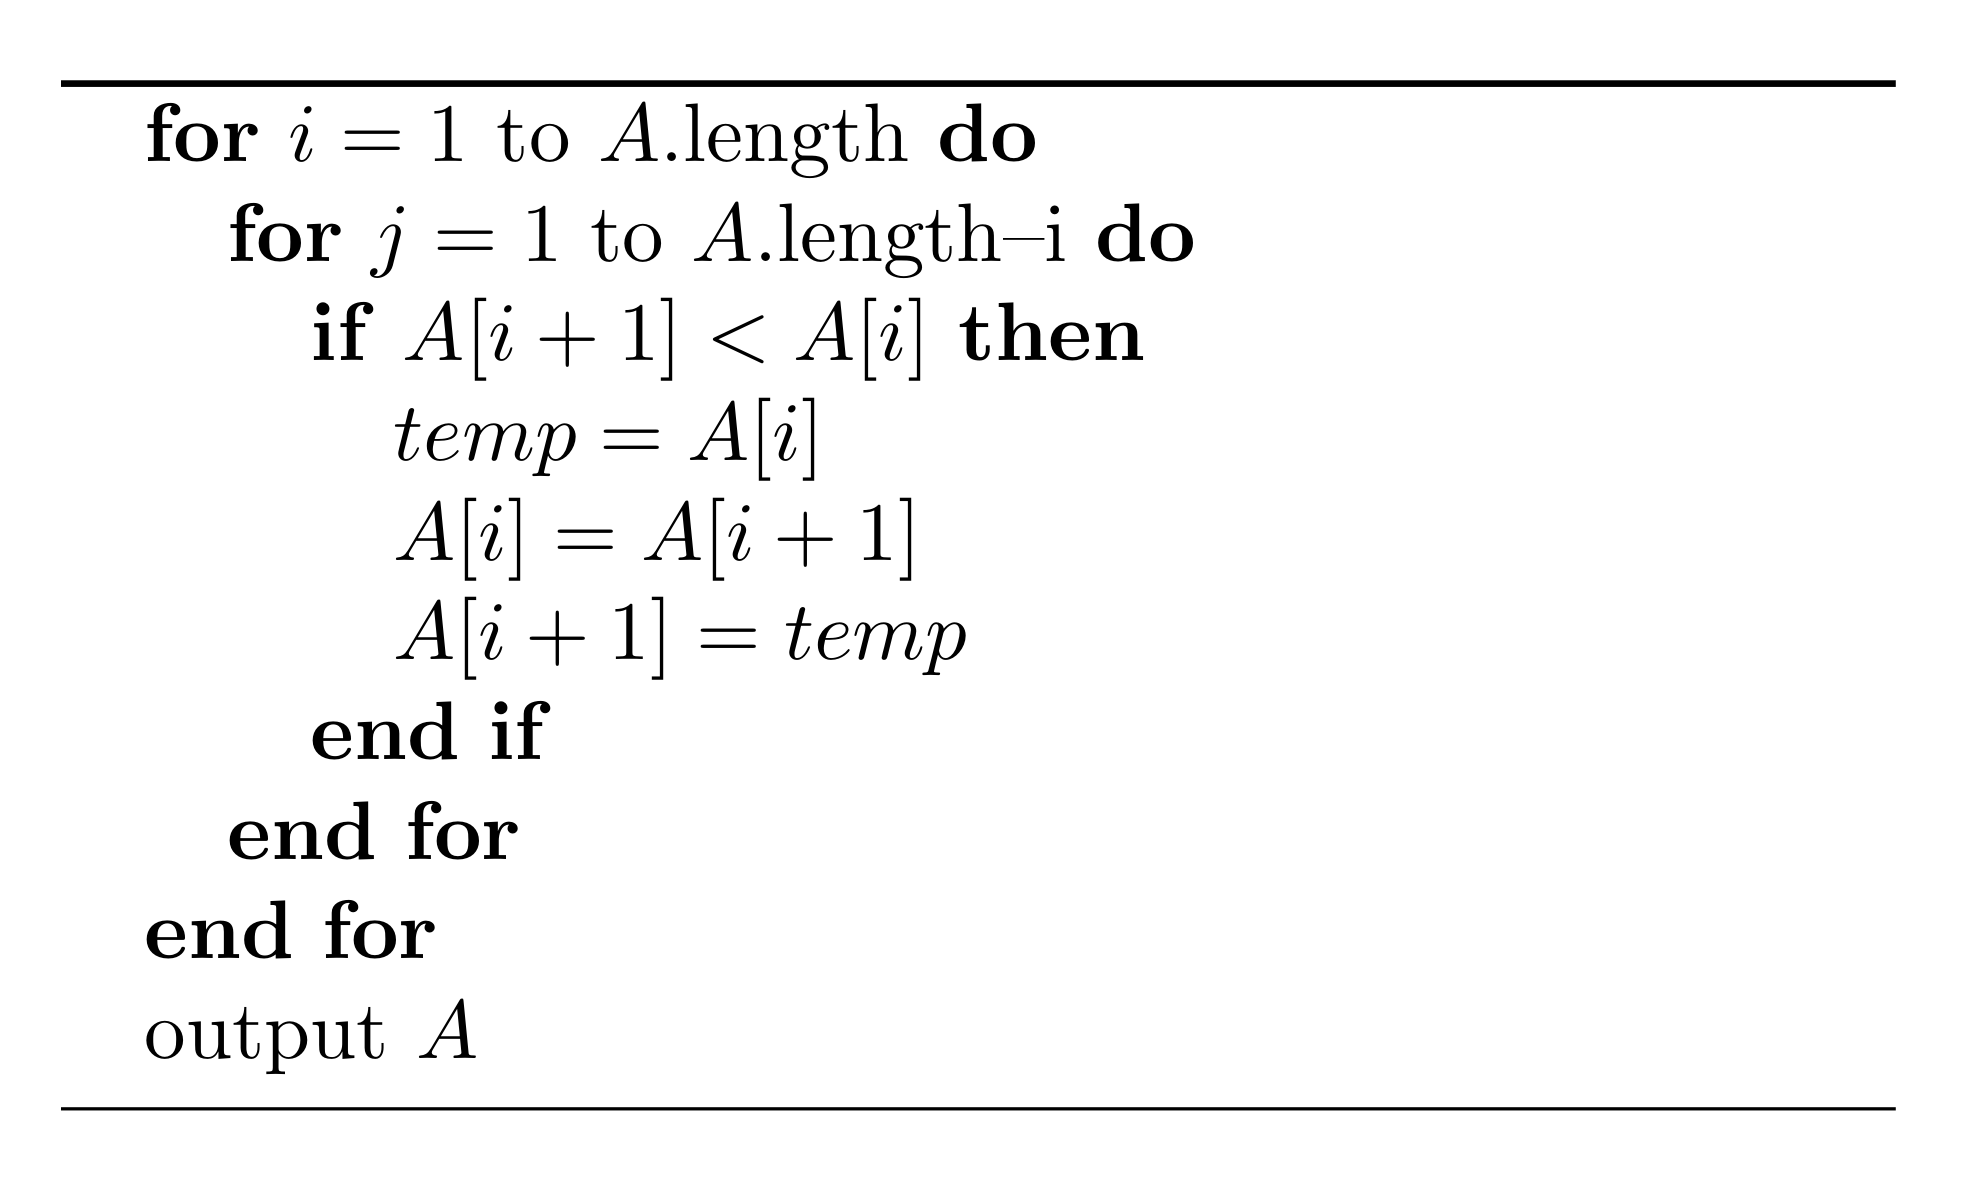
\includegraphics[width=0.25\textwidth]{algo.png}
\end{image}


% part 1 of question
\begin{question}
If the algorithm is invoked on the array $[ 5\quad 7\quad 3\quad 9]$ what is the output of the algorithm?
\begin{solution}
The output is 
\begin{matrix-answer}[name=M]
    correctMatrix = [['3','5','7','9']]
\end{matrix-answer}
\end{solution}

The output is:
$ [3 \quad 5 \quad 7 \quad 9] $
\end{question}

\begin{question}
% part 2 of question
What does the algorithm do? 
\begin{solution}
This algorithm \answer{sorts} the input array.
\end{solution}
This algorithm sorts the input array using a technique called bubble sort.
\end{question}

% part 3 of question
\begin{question}
Given an array with ten elements, how many comparisons (that is, $<$)
operations does the above piece of code perform?
\begin{solution}
There are \answer{45} comparisons.
\end{solution}  
The number of iterations of the inner loop starts with value 9 and
gradually decreases to 1. So the total number of comparisons is $ 9 +
8 + \ldots + 2 + 1 = 45$.
\end{question}

% part 4 of question
\begin{question}
Can you generalize your answer such that it gives an upperbound on the
number of comparison operations for an array of length $n$?
\begin{solution}
\begin{hint}
Are you familiar with asymptotic analysis of algorithms (especially
the Big-$\Theta$ notation)?
\end{hint}
The smallest upper bound (expressed as a function of $n$) is
\answer{$n^2$}.
\end{solution}
For an array of length $n$, the number of iterations of inner loop
starts with value $n-1$ and gradually decreases to 1. So the total
number of iterations would be $(n-1) + (n-2) + \ldots + 1 =
\frac{n(n-1)}{2}$. This indicates that the running time of this
algorithm is of $\Theta(n^2)$.
\end{question}


% Question 21
\begin{question}
What is the maximal number of leaves that a sorted binary tree with depth $4$ can possess?
\begin{solution}
The answer is \answer{16}.
\end{solution}
The maximal number of nodes at depth-level $d$ of a binary tree is $2^d$. So the answer to this question is $2^4 = 16$. 
\end{question}

% Question 22
\begin{question}
Order the following functions according to their growth-rate (use the theory of big-Oh notation). Put the slower growing functions first.
\[
n^7, 8n!, 5 \log_2 n,~ 3n, 2^n, ~ 7.5 n\log_2 n, ~ 6 n^2
\]
\begin{solution}
Specify the rank of each function. The rank of function with slowest growth is $1$ and rank of the fastest-growing one is $7$.
\begin{question}
$n^7$ \answer{5} 
\end{question}
\begin{question}
$8n!$ \answer{7} 
\end{question}
\begin{question}
$5 \log_2 n$ \answer{1} 
\end{question}
\begin{question}
$3n$ \answer{2} 
\end{question}
\begin{question}
$2^n$ \answer{6}  
\end{question}
\begin{question}
$7.5 n \log_2 n$ \answer{3}  
\end{question}
\begin{question}
$6 n^2$ \answer{4}
\end{question}

\end{solution}

This is the list of functions ordered according to their growth-rate:
\begin{equation*}
5 \log_2^n \prec 3n \prec 7.5 n \log_2{n} \prec 6n^2 \prec n^7 \prec 2^n \prec 8n!
\end{equation*}
\end{question}

\end{document}
